\documentclass{standalone}

\usepackage{tikz}

\begin{document}
  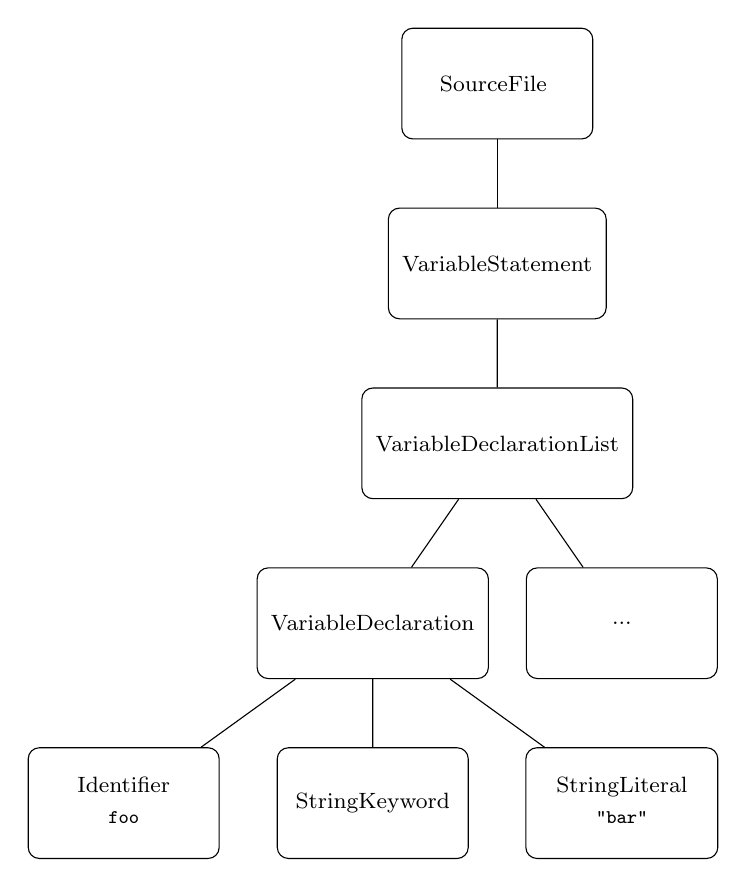
\begin{tikzpicture}[
    auto,
    sibling distance=9em,
    level distance=6.5em,
    font=\footnotesize,
    text centered,
    every node/.style = {
  	minimum width=6.9em,
  	minimum height=4em,
      shape=rectangle,
  	  rounded corners,
  	  inner xsep=.5em,
      draw,
  	  align=center
  	}
  ]
    
    \node { SourceFile }
      child { node {VariableStatement}
      child { node {VariableDeclarationList}
        child { node {VariableDeclaration}
        child { node {\begin{tabular}{c}Identifier\\[.2em]\centering\scriptsize{\texttt{foo}}\end{tabular}} }
        child { node {StringKeyword} }
        child { node {\begin{tabular}{c}StringLiteral \\[.2em]\centering\scriptsize{\texttt{"bar"}}\end{tabular}} }
      }
      child { node {...} }
      }
    };

  \end{tikzpicture}
\end{document}
